\documentclass{beamer}
\mode<presentation>
\usepackage{amsmath}
\usepackage{amssymb}
%\usepackage{advdate}
\usepackage{graphicx}
\graphicspath{{../figs/}}
\usepackage{adjustbox}
\usepackage{subcaption}
\usepackage{enumitem}
\usepackage{multicol}
\usepackage{mathtools}
\usepackage{listings}
\usepackage{url}
\def\UrlBreaks{\do\/\do-}
\usetheme{Boadilla}
\usecolortheme{lily}
\setbeamertemplate{footline}
{
  \leavevmode%
  \hbox{%
  \begin{beamercolorbox}[wd=\paperwidth,ht=2.25ex,dp=1ex,right]{author in head/foot}%
    \insertframenumber{} / \inserttotalframenumber\hspace*{2ex} 
  \end{beamercolorbox}}%
  \vskip0pt%
}
\setbeamertemplate{navigation symbols}{}
\let\solution\relax
\usepackage{gvv}
\lstset{
%language=C,
frame=single, 
breaklines=true,
columns=fullflexible
}

\numberwithin{equation}{section}



\begin{document}

\title{10.3.21}
\author{EE25BTECH11020 - Darsh Pankaj Gajare}
% \maketitle
% \newpage
% \bigskip
%\begin{document}
{\let\newpage\relax\maketitle}
%\renewcommand{\thefigure}{\theenumi}
%\renewcommand{\thetable}{\theenumi}


Question:\\
Find the point at which the line $y=x+1$ is a tangent to the curve $y^2=4x$.\\
\solution
The given conic can be expressed as
\begin{align}
	\vec{x}^\top \vec{V}\vec{x} + 2\vec{u}^\top\vec{x} + f = 0
\end{align}
where
\begin{align}
V = \myvec{0 & 0 \\ 0 & 1}, \quad
\vec{u} = \myvec{-2 \\ 0}, \quad
f = 0
\end{align}

The given line is 
\begin{align}
	\vec{n}^\top\vec{x}=C
\end{align}
where
\begin{align}
	\vec{n}=\myvec{-1\\1}, C=1
\end{align}
The eigenvector corresponding to the zero eigenvalue is
\begin{align}
	\vec{p_1}=\myvec{1\\0}
\end{align}
\begin{align}
	\myvec{\brak{\vec{u}+\kappa\vec{n}}^\top\\\vec{V}}\vec{q}=\myvec{-f\\\kappa\vec{n}-\vec{u}}
\end{align}
\begin{align}
	\kappa=\frac{\vec{p_1}^\top\vec{u}}{\vec{p_1}^\top\vec{n}}=\frac{\myvec{1&0}\myvec{-2\\0}}{\myvec{1&0}\myvec{-1\\1}}=2
\end{align}
\begin{align}
	\myvec{\brak{\myvec{-2\\0}+2\myvec{-1\\1}}^\top\\\myvec{0&0\\0&1}}\vec{q}=\myvec{0\\2\myvec{-1\\1}-\myvec{-2\\0}}
\end{align}
\begin{align}
	\myvec{-4&2\\0&0\\0&1}\vec{q}=\myvec{0\\0\\2}
\end{align}
Using augmented matrix,
\begin{align}
	\augvec{2}{1}{-4&2&0\\0&1&2}
\end{align}
$R_1=\frac{R_1-2R_2}{-4}$
\begin{align}
	\augvec{2}{1}{1&0&1\\0&1&2}
\end{align}
\begin{align}
	\vec{q}=\myvec{1\\2}
\end{align}
\begin{figure}[H]
	\centering
	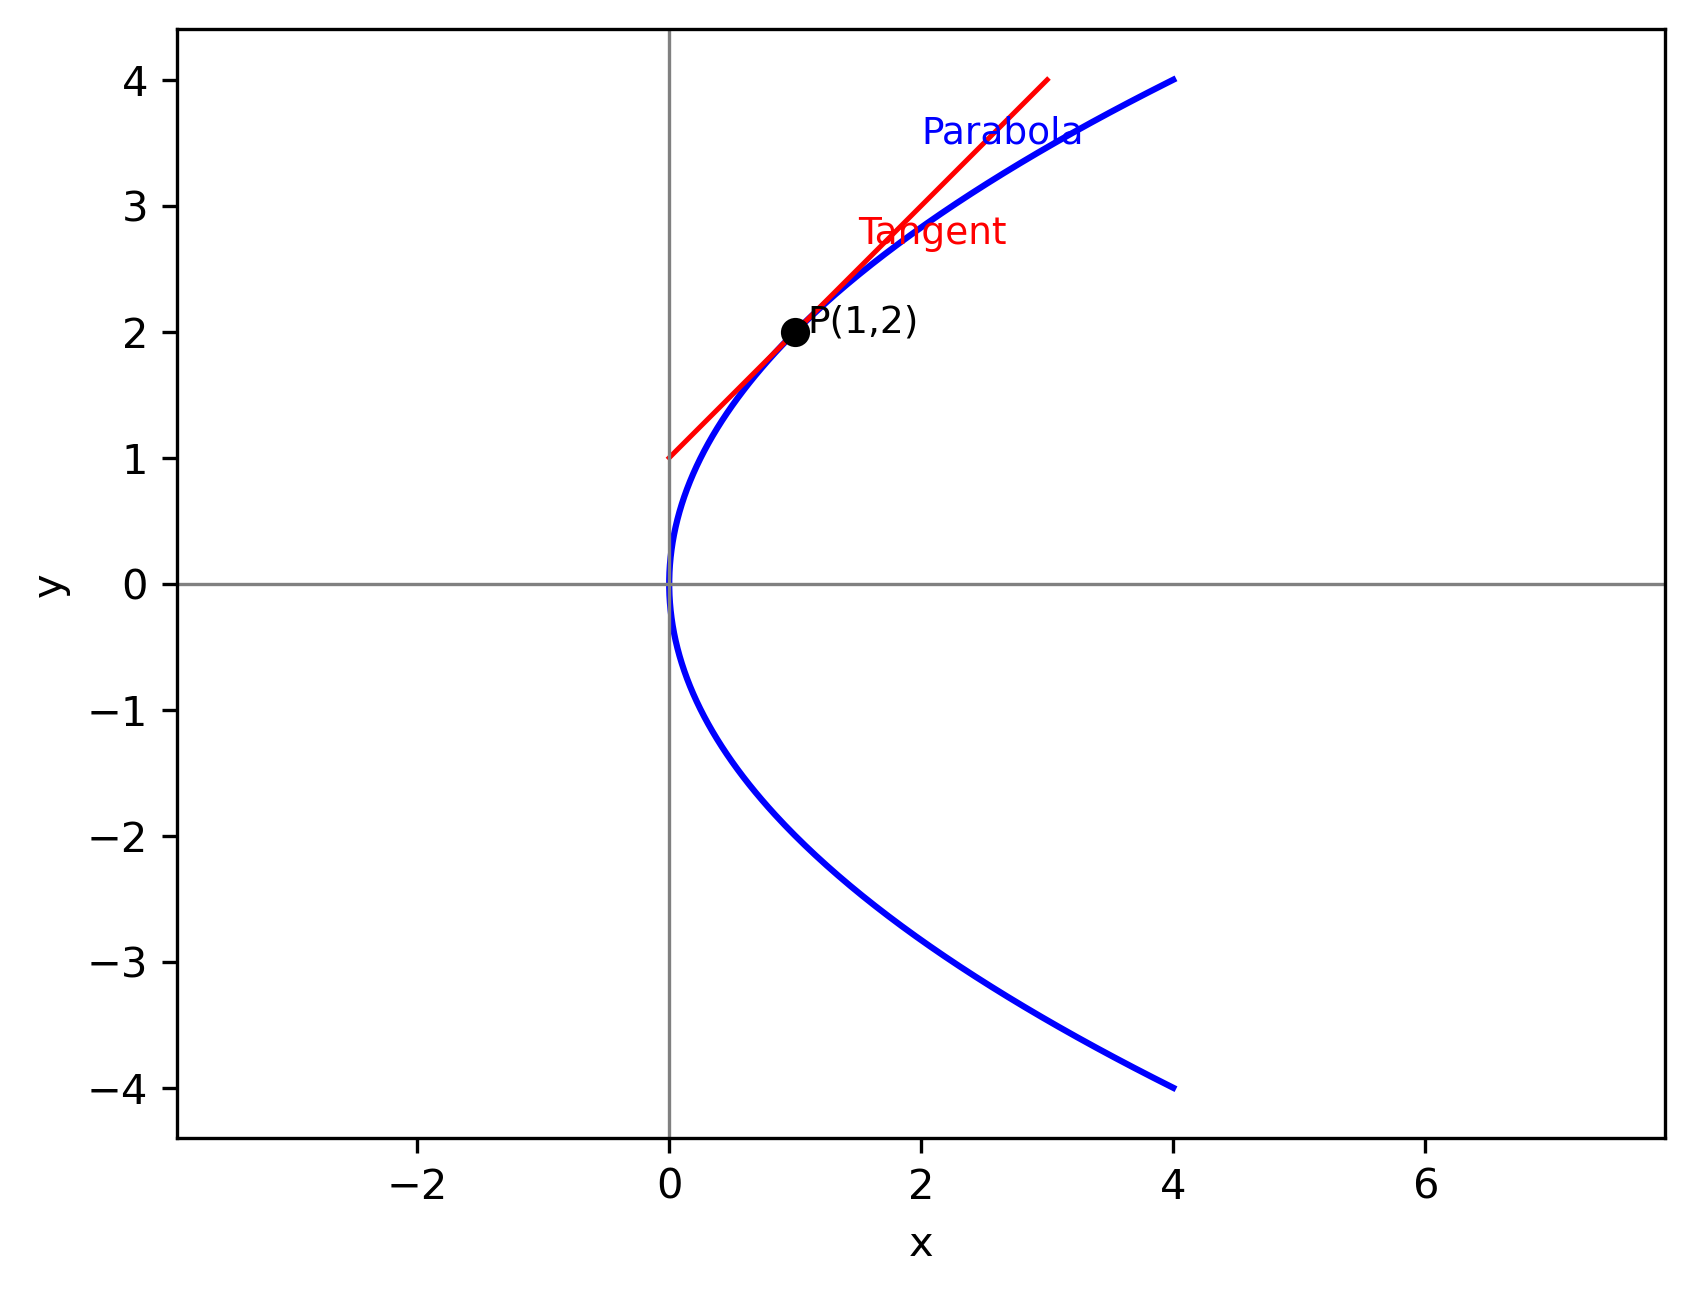
\includegraphics[scale=0.5]{img1}
	\caption*{Plot using C libraries:}
	\label{img1}
\end{figure}
\begin{figure}[H]
	\centering
	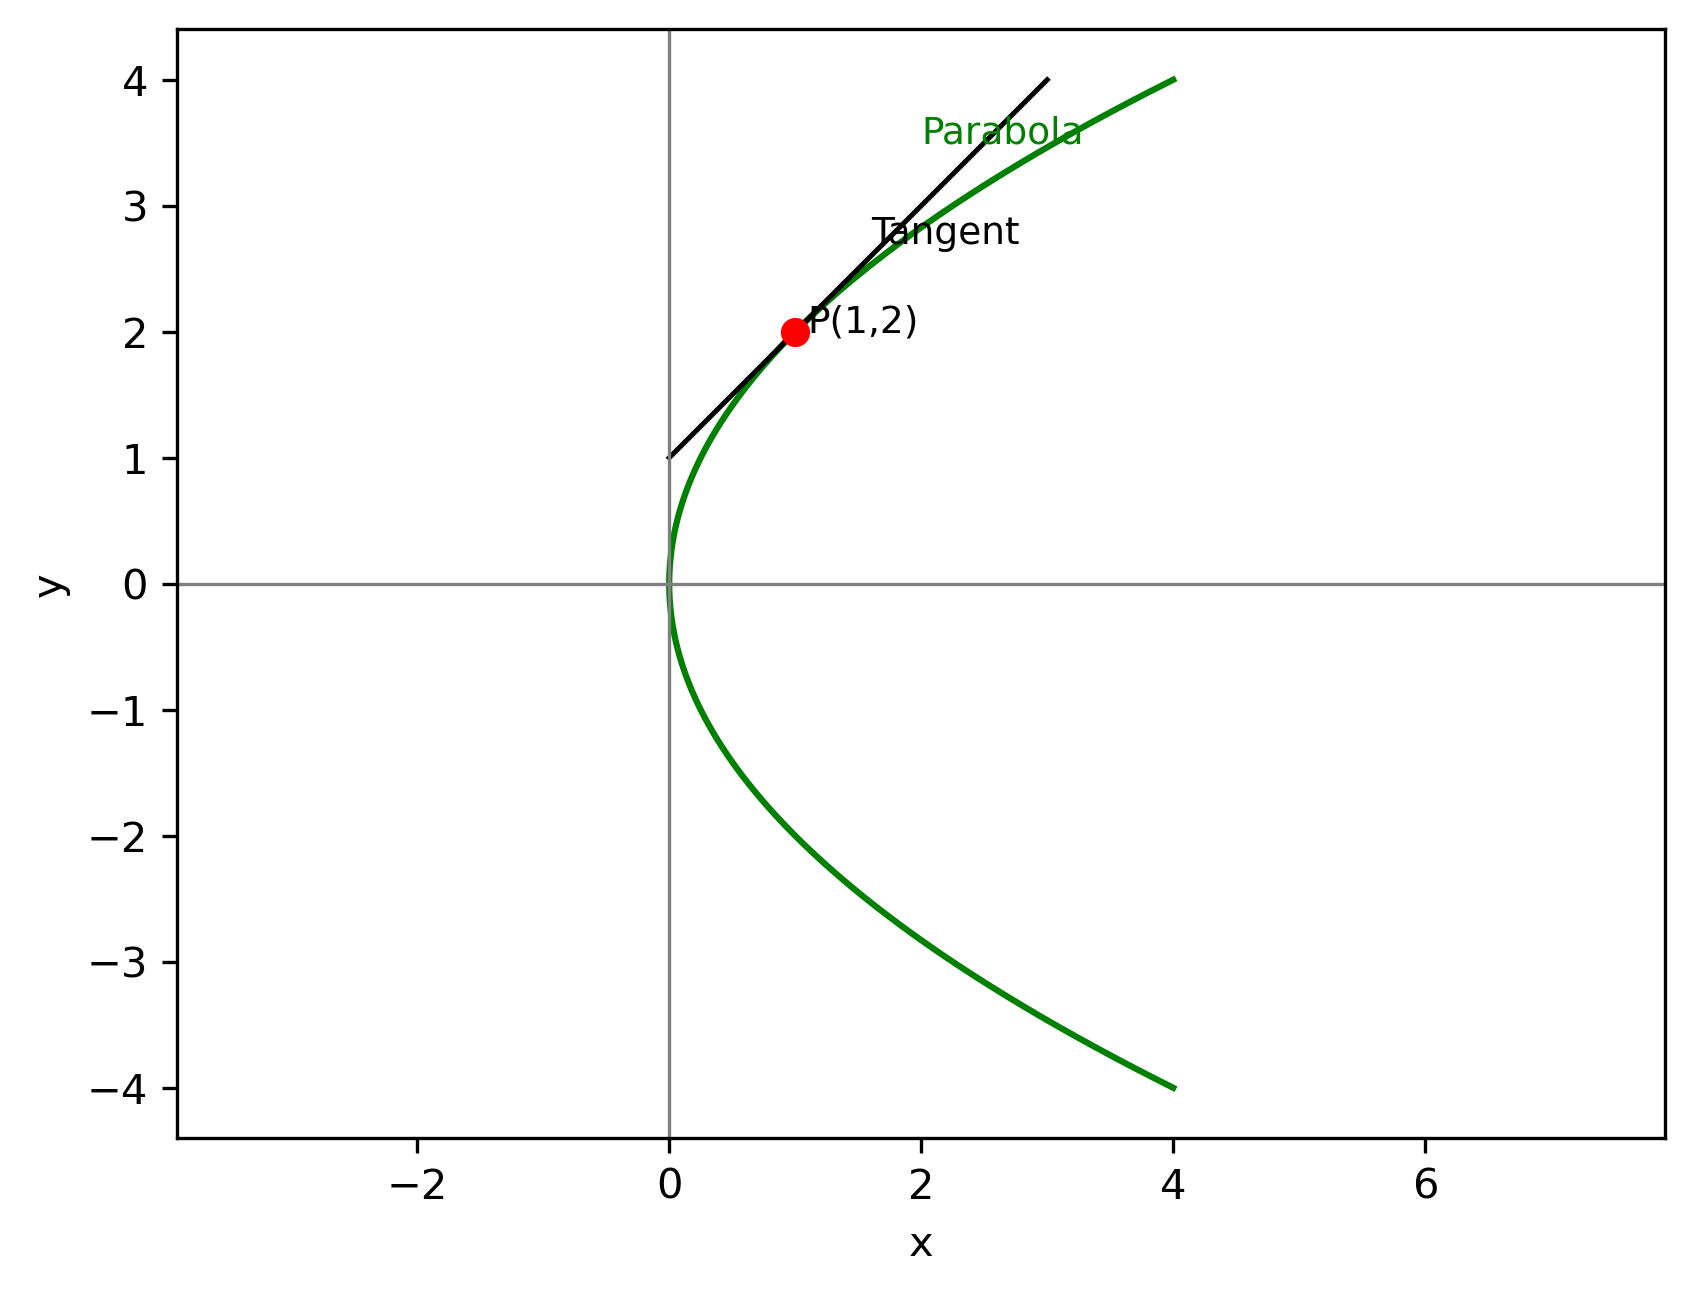
\includegraphics[scale=0.5]{img2}
	\caption*{
		Plot using Python:}
	\label{img2}
\end{figure}
\end{document}

